% !TEX encoding = UTF-8 Unicode

\documentclass[a4paper]{article}
\usepackage[T1]{fontenc} % da ne smara na linuxu


\usepackage{color}
\usepackage{url}
\usepackage[utf8]{inputenc} % make weird characters work
\usepackage{graphicx}
\usepackage{rotating} % slika rotirana

\usepackage[serbian]{babel}
%\usepackage[english,serbianc]{babel} %ukljuciti babel sa ovim opcijama, umesto gornjim, ukoliko se koristi cirilica

\usepackage[unicode]{hyperref}
\hypersetup{colorlinks,citecolor=green,filecolor=green,linkcolor=blue,urlcolor=blue}

%\newtheorem{primer}{Пример}[section] %ćirilični primer
\newtheorem{primer}{Primer}[section]

\begin{document}

\title{Crveno-crna stabla\\ \small{Seminarski rad u okviru kursa\\Konstrukcija i analiza algoritama 2\\ Matematički fakultet}}

\author{Nikola Dimitrijević, 1086/2017\\ nikoladim95@gmail.com}
\maketitle

\abstract{
    Crveno-crna stabla su vrsta binarnih samobalansirajućih stabala. To je struktura podataka koja garantuje brze operacije umetanja, pretrage i brisanja.
    Svaki čvor stabla ima boju: crnu ili crvenu. Uz određena pravila i načine na koje se menja stablo dobija se gornja granica za koliko stablo može biti nebalansirano.

}

\tableofcontents

\newpage

\section{Osnovno}
\label{sec:uvod}
Crveno-crna stabla su struktura podataka koja omogućava brze operacije umetanja, brisanja i pretrage. Spadaju u binarna samobalansirajuća stabla.
Svaki čvor ima dodatan bit (ili već neki tip podatka) koji reprezentuje boju čvora. Autori su se odlučili za crvenu i crnu boju jer je, pored klasične crne,
crvena najbolje izgledala na tadašnjim laserskim štampačima \cite{funfact}. Još jedan razlog je to što su imali crvene i crne hemijske pa su tako crtali ova stabla.

\begin{figure}[h!]
\begin{center}
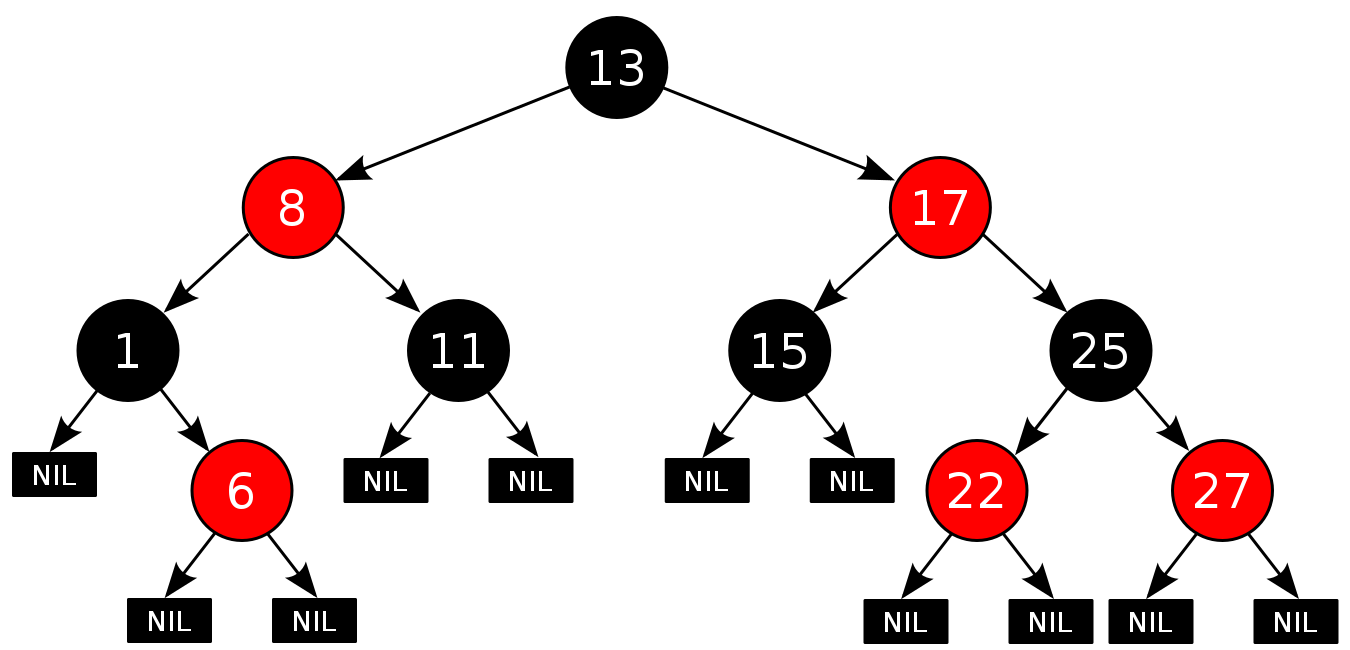
\includegraphics[scale=0.2]{example.png}
\end{center}
\caption{Primer crveno-crnog stabla}
\label{fig:primer}
\end{figure}

Za razliku od mnogih stabala, u implementacijama crveno-crnih stabala se umesto uobičajenih null pokazivača koriste specijalni null čvorovi (Na slici \ref{fig:primer} su označeni sa NIL) koji ne sadrže nikakve podatke
koji se unose u strukturu. Iako je moguće implementirati sve operacije crveno-crnih stabala korišćenjem običnih null pokazivača, ovako se uprošćavaju njihove implementacije.
Da bi se uštedelo na memoriji, umesto da postoji mnogo različitih null čvorova, moguće je imati jedan takav čvor u memoriji, a da svi ostali koji žele da pokazuju na null čvor pokazuju
baš na samo tog jednog.
Crveno-crna stabla se koriste za skladištenje podataka koji imaju uređenost, pošto se na osnovu poretka određuje pozicija elemenata u stablu.
\section{Svojstva}
\label{sec:svojstva}

\begin{itemize}
        \item Svaki čvor je ili crn ili crven.
        \item Koren je crn.
        \item Svi listovi su crni.
        \item Ako je čvor crven, onda su mu oba sina crna.
        \item Svaki put od korena do svih NIL listova ima isti broj crnih čvorova.
\end{itemize}

Na osnovu datih svojstava može se i intuitivno pokazati zašto ova stabla ostaju balansirana.

Svaki put od korena do lista ima isti broj crnih čvorova. Jedini način da se poveća broj čvorova na 
tom putu jeste da se ubace crveni čvorovi. Međutim, kako ne smeju biti dva crvena čvora jedan za drugim,
to znači da se bilo koja putanja od korena do lista može udvostručiti ako bi se nakon svakog crnog čvora
ubacio crven čvor. To bi u najgorem slučaju udvostručilo visinu tog podstabla, ali je upravo to i najviše
što stablo može biti udaljeno od potupne balansiranosti. Dakle u najgorem slučaju je jedno podstablo dva puta
dublje od svog brata podstabla.

\textit{Crna dubina} stabla je broj crnih čvorova od korena do listova, koji je za svaki put od korena do lista isti.

\section{Operacije}


\subsection{Pretraga}

Počevsi od korena, ako je trenutni čvor trazen: gotovo, inače ako
je traženi manji od trenutnog rekurzivno se pretražuje levo podstablo, inače se rekurzivno pretražuje desno podstablo.

\subsection{Umetanje}
\textit{Deda} čvora je od čvorovog oca otac.

\textit{Ujak} čvora je od dede čvora drugi sin, odnosno onaj sin koji nije roditelj čvoru.


    Trougao formacija je kada je čvor levi sin oca, a otac desni sin dede, ili slučaj u ogledalu. 
    Primer na slici \ref{fig:triangle}.
    \begin{figure}[h!]
        \begin{center}
        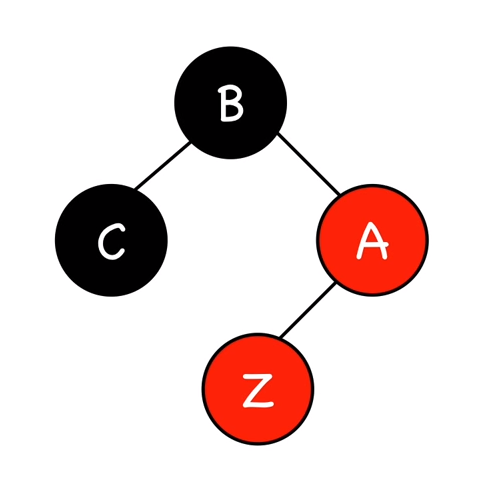
\includegraphics[scale=0.5]{triangle.png}
        \end{center}
        \caption{Trougao formacija.}
        \label{fig:triangle}
    \end{figure}

    Linija formacija je kada je čvor levi sin oca i otac levi sin dede, ili u slučaj ogledalu.
    Primer na slici \ref{fig:line}.
    \begin{figure}[h!]
        \begin{center}
        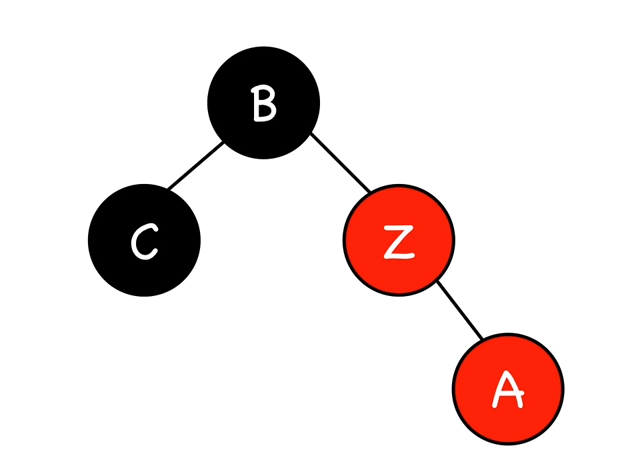
\includegraphics[scale=0.5]{line.png}
        \end{center}
        \caption{Linija formacija.}
        \label{fig:line}
        \end{figure}

    Postupak umetanja:
    \begin{itemize}

    \item Kada se dodaje nova vrednost u stablo, uvek se prvo nov čvor oboji u crveno.
    \item Spušta se kroz stablo do listova, i onda se umeće kao potomak.

    \item Ako je roditelj crn, onda kraj

   \item Ako je novi čvor koren, oboji ga u crno.
   \item Ako mu je otac crn, onda se ne radi ništa, jer je stablo i dalje ispravno.
   \item Ako mu je ujak crven, onda oboji ujaka i oca u crno, a dedu u crveno. Obradi dedu rekurzivno.
   \item Ako mu je ujak crn i u trouglu su, onda se rotira otac čvora u suprotnu stranu od sina.
   \item Ako mu je ujak crn i u liniji su, onda se deda čvora rotira u suprotnu stranu od unuka.
\end{itemize}


\subsection{Brisanje}
Brisanje je komplikovanije od pretrage i umetanja.

\begin{itemize}
    \item Prvo se traži čvor koji se briše. Ako nije prisutan kraj.
    \item Ako nađeni čvor ima oba sina, onda prvo mora da se svede na prostiji slučaj, gde ima 0 ili 1 sina.
    \item Nađe se sledbenik trenutnog čvora u stablu, odnosno najmanji element u desnom podstablu.
    \item Čvor koji se briše zameni mesto sa njegovim sledbenikom.
    \item Njegov sledbenik ima najviše jednog potomka, pošto da je imao levog potomka, onda bi on bio sledbenik.
    \item Sada čvor koji se briše ima najviše jednog potomka. 
    \item Ako nema nijednog potomka i crven je čvor, onda se samo obriše.
    \item Inače, pošto je čvor crn ne može samo da se obriše jer bi se smanjila crna dubina.
    \item Ako čvor ima jedno crveno dete, umesto sebe stavi dete i obriše sebe.
    \item Inače se prolazi kroz šest specifičnih i zamršenih koraka. Za detalje pogledati \cite{cases}.
\end{itemize}


\section{Upoređivanje sa AVL stablima}
    Crveno-crna stabla su, kao i AVL stabla, samobalansirajuća. Oba pružaju $O(log n)$ vreme pretrage, umetanja i brisanja.
    AVL stabla su bila popularna pre nego što su crveno-crna stabla postala poznata.

    Za razliku od AVL stabla, teža su za implementaciju. Pre svega zbog svih detalja implementacije šest različitih slučajeva 
    popravke nakon brisanja.
    Oba stabla imaju linearnu memorijsku složenost.

    AVL stabla imaju jaču garanciju balansiranosti. Kod njih je razlika dubina levog i densog podstabla najviše jedan, a crveno-crna garantuju da razlika nije više od duplo.

    Prednost crveno-crnih stabla je što garantuju $O(1)$ rotacija po operaciji umetanja. 
    Ta stvar zaista utiče na performanse u pravim implementacijama.

    Crveno-crna stabla garantuju da jedna strana stabla nije više od duplo duža od druge.

    AVL stabla imaju 4 rotacije. LR, LL, RR, RL.
    Crveno-crna stabla imaju samo levu i desnu rotaciju. Međutim, postoje neki slučajevi kada se briše element u kojima je potrebna dodatna obrada
    kako bi stablo ostalo balansirano.
    Ima 6 mogućih slucajeva. Ide se od prvog do poslednjeg, usput primenjujući pravila ako je moguće. Postoje tri terminirajuća pravila, tj. 
    ako je njihov uslov zadovoljen, onda se odradi potrebno ažuriranje i prekida prolazak kroz ostale slučajeve.
    
    Pošto su i crveno-crno stablo i AVL stablo stabla pretrage, na uobičajen način se vrši pretraga.

\subsection{Zaključak}
Crveno-crna stabla su danas najpopularniji izbor implementacije samobalansirajućih binarnih stabala.

Primeri korišćenja crveno-crnih stabala:
\begin{itemize}
    \item  Java: java.util.TreeMap, java.util.TreeSet
    \item C++ STL: map, multimap, multiset \cite{gcc}
    \item Linux jezgro: Potpune fer raspoređivač, linux/rbtree.h
    \item U funkcionalnom programiranju za implementaciju postojanih struktura podataka. Tada svaka operacija brisanja i umetanja ima dodatnu memorijsku složenost O(log n) kako bi moglo da se rekonstruišu ranija stabla \cite{persistent}.
\end{itemize}

Na slici \ref{fig:chart} je nacrtan grafik na kome se vidi vreme  izvršavanja algoritma za različite ulaze.
Ulaz označava koliko će se nasumičnih brojeva ubaciti u stablo.
Vreme izvršavanja počinje da bude osetno tek za ulaze od oko 90000.
Za veće ulaze se jasnije vidi kako raste potrebno vreme. Kada je u pitanju
ulaz veličine pola miliona tada je potrebno 11 sekundi, a za milion 25 sekundi.
To je tek nešto sporije od očekivanog odnosa vremena za algoritam linearne složenosti, što je 
razuman reuzltat s obzirom da je složenost ubacivanja $n$ elemenata $O(n logn)$.

\begin{sidewaysfigure}[ht]
    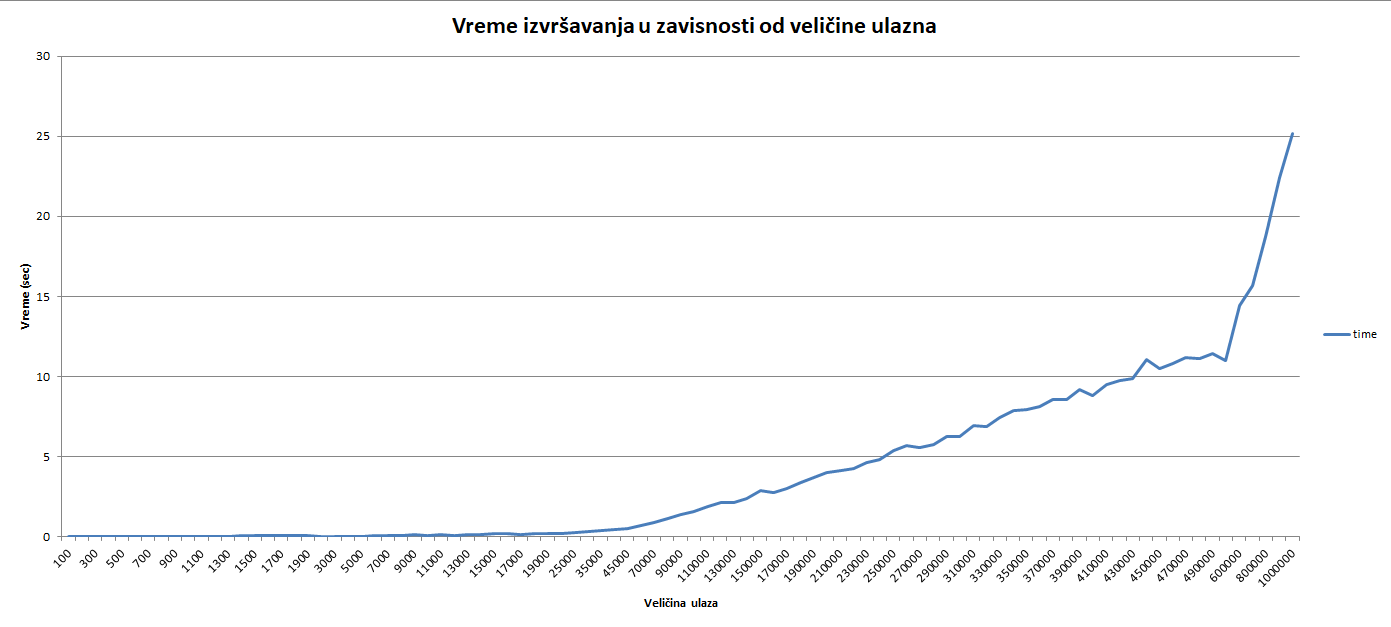
\includegraphics[width=\textwidth]{chart.png}
    \caption{Testiranje algoritma, skala x ose raste brže od linearno.}
    \label{fig:chart}
\end{sidewaysfigure}

\addcontentsline{toc}{section}{Literatura}
\appendix
\bibliography{seminarski} 
\bibliographystyle{plain}



\end{document}
